\providecommand{\pdfxopts}{a-1b,cyrxmp}
\providecommand{\thisyear}{2020}
\immediate\write18{rm \jobname.xmpdata}%  uncomment for Unix-based systems
\begin{filecontents*}{\jobname.xmpdata}
\Title{Силовая электроника. Практическая работа №2\textemdash\thisyear}
\Author{Артем Николаевич Прокшин}
\Creator{pdfTeX + pdfx.sty with options \pdfxopts }
\Subject{Практическая работа №2
\sep
        Варианты построения силовых схем преобразователей
\sep
	питаемых от 3-фазной сети}
\Keywords{силовые преобразователи, варианты силовых схем преобразователей, ЛЭТИ}
\CoverDisplayDate{май \thisyear}
\CoverDate{2020-05-23}
\Copyrighted{True}
\Copyright{Public Domain}
\CopyrightURL{http://github.com/trot-t}
\Creator{pdfTeX + pdfx.sty with options \pdfxopts }
\end{filecontents*}

\documentclass{article}

\pdfcompresslevel=9

\usepackage[\pdfxopts]{pdfx}[2016/03/09]
\PassOptionsToPackage{obeyspaces}{url}
\let\tldocrussian=1  % for live4ht.cfg


%\usepackage{extsizes}
\usepackage[left=15mm, top=20mm, right=15mm, bottom=20mm, nohead, footskip=7mm]{geometry} % настройки полей документа

\usepackage[T2A]{fontenc}
\usepackage[utf8]{inputenc}
\usepackage[english,russian]{babel}
\usepackage{tikz}
\usepackage[european,cuteinductors,smartlabels]{circuitikz}
\title{Практическая работа №2}
%\author{студент:    группы    }
% Конец преамбулы
\begin{document}
\maketitle

\section*{Варианты построения силовых схем преобразователей, преобразователей, питаемых от 3-фазной сети, с разным эквивалентным числом фаз}
\begin{figure}[!ht]
\begin{tabular}{cccc}
\begin{minipage}{0.22\textwidth}
	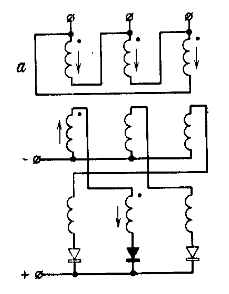
\includegraphics[scale=0.3]{schema1}
	\caption{\small Нулевая схема: треугольник -- звезда}
\end{minipage}
	&
\begin{minipage}{0.22\textwidth}
        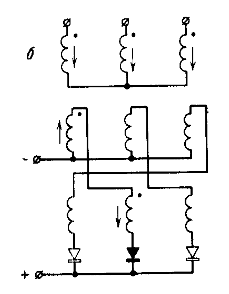
\includegraphics[scale=0.3]{schema2}
	\caption{\small Нулевая схема: звезда -- звезда}
\end{minipage}
        &
\begin{minipage}{0.25\textwidth}
        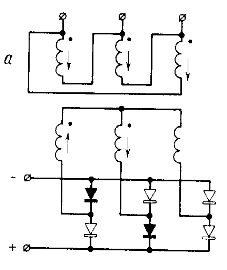
\includegraphics[scale=0.3]{schema3}
	\caption{\small Мостовая схема (Ларионова): треугольник -- звезда}
\end{minipage}
        &
\begin{minipage}{0.22\textwidth}
%        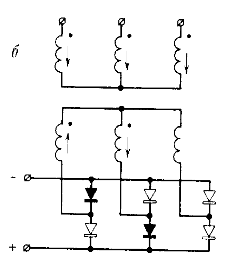
\includegraphics[scale=0.3]{schema4}
	\begin{circuitikz}[scale=0.3]
\ctikzset{bipoles/americaninductor/coils=3} %  3 витка
\ctikzset{bipoles/diode/width=0.1}
\ctikzset{bipoles/diode/height=0.1}
\ctikzset{bipoles/americaninductor/height=0.24}
\ctikzset{bipoles/americaninductor/coil height=0.05}
\ctikzset{bipoles/americaninductor/width=0.24}
\ctikzset{nodes width/.initial=.02}

\draw (3,8) to[american inductor,o-] (3,5.5);
\draw[fill] (3.25, 7.5) circle (2pt);
\draw (4.5,8) to[american inductor,o-*] (4.5,5.5); %-* соединение
\draw[fill] (4.75, 7.5) circle (2pt);
\draw (6,8) to[american inductor,o-] (6, 5.5);
\draw[fill] (6.25, 7.5) circle (2pt);
\draw (3,5.5) -- (6,5.5);

\draw[fill] (2.6,4.97) rectangle (6.4,5.03);

\draw (3,4.5) to[american inductor] (3,2) node(a){}; % node[above left]{\small{a}};
\draw[fill] (3.25, 2.5) circle (2pt);
\draw (4.5,4.5) to[american inductor,*-] (4.5,2) node(b){}; % node[above left]{\small{b}};
\draw[fill] (4.75, 2.5) circle (2pt);
\draw (6,4.5) to[american inductor] (6,2) node(c){}; % node[above left]{\small{c}};
\draw[fill] (6.25, 2.5) circle (2pt);
\draw (3,4.5) -- (6,4.5);

\draw(3.75,-0.5) to[D-] (3.75,1) node(v1){};
\draw(3.75,-2) node(v4){} to[D-, -*] (3.75,-0.5) node(na) {};
        \draw (a.center) |- (na.center);
\draw(5.25,-0.50) to[D-,-*] (5.25,1);
\draw(5.25,-2) to[D-, *-*] (5.25,-0.5) node(nb) {};
        \draw (b.center) |- (nb.center);
\draw(6.75,-0.5) to[D-,-*] (6.75,1);
\draw(6.75,-2) to[D-, *-*] (6.75,-0.5) node(nc) {};
        \draw (c.center) |- (nc.center);
\draw (v1.center) to[short,-o] ++ (4,0) node[right](plus){\tiny{+}};
\draw (v4.center) to[short,-o] ++ (4,0) node[right](minus){-};
\end{circuitikz}


	\caption{\small Мостовая схема (Ларионова): звезда -- звезда}
\end{minipage}
       \\
\begin{minipage}{0.22\textwidth}
        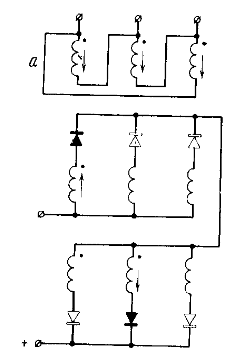
\includegraphics[scale=0.3]{schema5}
	\caption{\small последовательная схема (Вологдина): треугольник -- две звезды}
\end{minipage}
        &
\begin{minipage}{0.22\textwidth}
        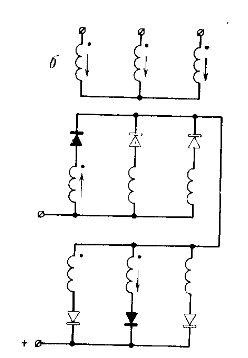
\includegraphics[scale=0.3]{schema6}
	\caption{\small последовательная схема (Вологдина): звезда -- две звезды}
\end{minipage}
        &
\begin{minipage}{0.25\textwidth}
        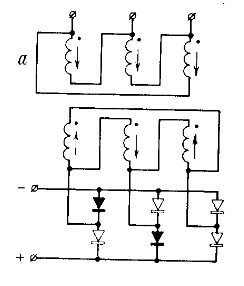
\includegraphics[scale=0.3]{schema7}
	\caption{\small Мостовая схема: треугольник -- треугольник}
\end{minipage}
        &
\begin{minipage}{0.22\textwidth}
        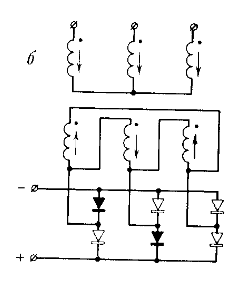
\includegraphics[scale=0.3]{schema8}
	\caption{\small Мостовая схема: звезда -- треугольник}
\end{minipage}
       \\
\begin{minipage}{0.22\textwidth}
        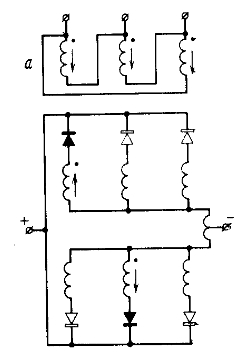
\includegraphics[scale=0.3]{schema9}
	 \caption{\small Параллельная схема (Кюблера): треугольник -- две звезды}
\end{minipage}
        &
\begin{minipage}{0.22\textwidth}
        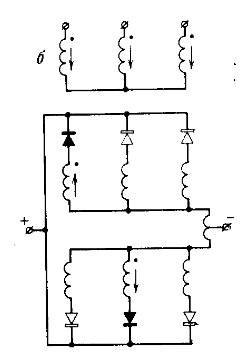
\includegraphics[scale=0.3]{schema10}
	\caption{\small Параллельная схема (Кюблера): звезда -- две звезды}
\end{minipage}
        &
\begin{minipage}{0.25\textwidth}
        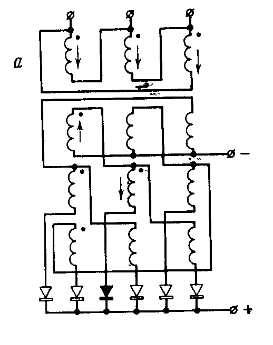
\includegraphics[scale=0.3]{schema11}
	\caption{\small Нулевая схема: треугольник -- двойной зигзаг}
\end{minipage}
        &
\begin{minipage}{0.22\textwidth}
        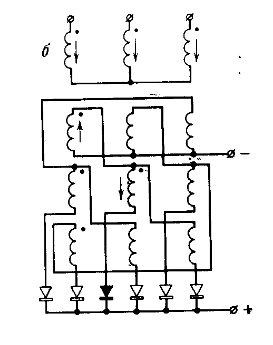
\includegraphics[scale=0.3]{schema12}
	\caption{\small Нулевая схема: звезда -- двойной зигзаг}
\end{minipage}
       \\
\end{tabular}
\end{figure}


\section*{Задание}
\begin{itemize}
	\item Изобразить схему согласно варианта на рис 1-12 (схема должны быть редактируемой в Компасе или \LaTeX \cite{circuitikz}, элементы схемы в векторном виде -- при изменении размера изображение не должно деградировать);
	\item изобразить вектора фаз первичной обмотки трансформатора, вторичной обмотки трансформатора для выбранного момента времени;
	\item построить график выпрямленного напряжения для одного периодa.

\end{itemize}



\section*{Примеры}

Редактирование можно выполнить \href{overleaf.com}{онлайн}.
Зарегистрироваться и создать новый проект.



Внутри тегов $\backslash begin\{document\}$ и $\backslash end\{document\}$ вставляем: 

\begin{verbatim}
\begin{circuitikz}
\ctikzset{bipoles/americaninductor/coils=3} % для красоты используем 3 витка
\draw (0,0) to[american inductor,o-*] (3,0); % o- это контакт; -* это соединение
\end{circuitikz}
\end{verbatim}


\begin{circuitikz}
\ctikzset{bipoles/americaninductor/coils=3} 
\draw (0,0) to[american inductor,o-*] (3,0); 
\end{circuitikz}

\textcolor{red}{последний символ команды $\backslash draw$ должен быть точка с запятой ;}

\begin{verbatim}
\draw (0,0) node[above]{+} to[american inductor,o-*] (3,0); % плюс над точкой (0,0); -* соединение
\draw[fill] (1.85, 0.4) circle (1.5pt); % точка возле катушки
\end{verbatim}

\begin{circuitikz}
\ctikzset{bipoles/americaninductor/coils=3}
\draw (0,0) node[above] {+} to[american inductor] (3,0); % плюс над контактом  в точке (0,0)
\draw[fill] (2.25, 0.15) circle (1.5pt);
\end{circuitikz}

Для указания начало обмотки используют точку \cite{UGOinductor}.

Позицию символа относительно точки (x,y) можно задать как (x,y) node[below right] \{символ\} и т.п. \cite{circuitikz}

\begin{verbatim}
\begin{circuitikz}
\draw (0,-1) to[D-] (3,-1) node[right] {диод по ГОСТу};
\end{circuitikz}
\end{verbatim}

\begin{circuitikz}
%\draw (0,0) to[D] (3,0) node[right] {диод}; это не нужно использовать
\draw (0,-1) to[D-] (3,-1) node[right] {диод по ГОСТу};
%\draw (0,-2) to[D*] (3,-2) node[right] {закрашенный диод}; это не нужно использовать
\end{circuitikz}


Если размер диодов хотим уменьшить

\begin{verbatim}
\begin{circuitikz}
\ctikzset{bipoles/diode/width=0.2,bipoles/diode/height=0.2}
\draw (0,0) to[D-] (3,0) node[right] {}; %справа объявили узел(node) ничего не написав {}
\draw (0,-0.7) to[D-] (3,-1); % если метка не нужна, то node {} не нужна
\end{circuitikz}
\end{verbatim}

\begin{circuitikz}
\ctikzset{bipoles/diode/width=0.2,bipoles/diode/height=0.2}
\draw (0,0) to[D-] (3,0) node[right] {}; 
\draw (0,-0.7) to[D-] (3,-0.7);
\end{circuitikz}



\subsection*{Пример графика:}

\begin{verbatim}
\begin{tikzpicture}[scale=0.67]
\draw[thin, ->] (-6,0) -- (6,0) node[right] {$\omega t$}; % чертим ось x
\draw[thin, ->] (0,-1.5) -- (0,1.5) node[left] {$U$};  % чертим ось y
 \draw[domain=-5:0, help lines, smooth] % график для интервала -5:0
        plot ({\x},{sin(\x*180/3.14)}); % фунция sin имеет аргумент в градусах
 \draw[domain=0:5, help lines, smooth]  % график для интервала 0:5
        plot ({\x},{cos(\x*180/3.14)});
\end{tikzpicture}
\end{verbatim}

\begin{figure}[ht!]
\centering
\begin{tikzpicture}[scale=0.67]
%\newcommand{\xb}{-3} % введем переменную \xb равную -3
%\newcommand{\xa}{3}
\draw[thin, ->] (-6,0) -- (6,0) node[right] {$\omega t$}; % чертим ось x
\draw[thin, ->] (0,-1.5) -- (0,1.5) node[left] {$U$};  % чертим ось y
% % подписи под точками на оси
%\foreach \x\xtext in {-5/-5,5/5,{\xb}/\xb,{\xa}/{\gamma}} %
%   \draw (\x,0.1) -- (\x,-0.1) node[below] {$\xtext$};
% % строим график
 \draw[domain=-5:0, help lines, smooth] % график для интервала -5:0
        plot ({\x},{sin(\x*180/3.14)}); % фунция sin имеет аргумент в градусах
 \draw[domain=0:5, help lines, smooth]  % график для интервала 0:5
        plot ({\x},{cos(\x*180/3.14)});
\end{tikzpicture}
	\caption{Пример вычерчивания графика}
\end{figure}

\renewcommand{\bibname}{}
\begin{thebibliography}{5}
	\bibitem{trans}	\href{http://docs.cntd.ru/document/gost-16772-77}{ГОСТ 16772-77} Трансформаторы и реакторы преобразовательные. Общие технические условия
	\bibitem{UGOdiod} \href{https://znaytovar.ru/gost/2/GOST_273073_ESKD_Oboznacheniya.html}{ГОСТ 2.730-73}  Единая система конструкторской документации. Обозначения условные графические в схемах.  Приборы полупроводниковые
	\bibitem{UGOinductor} \href{http://docs.cntd.ru/document/1200006612} {ГОСТ 2.723-68}Единая система конструкторской документации (ЕСКД). Обозначения условные графические в схемах. Катушки индуктивности, дроссели, трансформаторы, автотрансформаторы и магнитные усилители (с Изменениями N 1, 2, 3)   
	\bibitem{bulgakovAA} Булгаков, А.А. Новая теория управляемых выпрямителей, Москва, Наука, 1970. -- 320с.
        \bibitem{circuitikz} \href{http://texdoc.net/texmf-dist/doc/latex/circuitikz/circuitikzmanual.pdf}{Описание пакета \LaTeX для черчения электрических схем для статей и публикаций}
\end{thebibliography}

\end{document}
